\chapter{Concept and Design}
\label{cha:conceptanddesign}
The goal of this bachelor's thesis is the development of an app for mobile devices, which provides students at TU Berlin the possibility to navigate and inform themselves about their campus in Charlottenburg. The main concept of the mobile app is inspired by popular smartphone navigation systems such as Google or Apple Maps and focuses on mapping TU Berlin's main campus and the most important web resources connected to it onto a single digital map.

\section{Key features and technologies}
The following sections provide a detailed overview of the app's key features and the underlying technologies used in this thesis.

\subsection{Digital map of campus Charlottenburg}
The main element of the mobile app consists of a locally implemented map of TU Berlin's central campus in Charlottenburg. It provides the user a manageable overview of TU Berlin's buildings, pathways, green areas as well as its surrounding environment. The following table displays possible map features with a description of their relevance for the mobile app:\\

\begin{longtable}{|p{1.0in}|p{5.0in}|}
    \hline
    Feature & Description and relevance \\
    \hline
    All buildings of TU Berlin & To provide the user the ability to easily locate the buildings of TU Berlin, all facilities connected to the university need to be specially highlighted on the map. The buildings of TU Berlin are therefore the most important map feature.\\
    \hline
    All pathways on campus & Footwalks and cycleways that lay on the campus are important for the navigation system of the mobile app. To prevent the map from being cluttered, a hierarchy must be established between important pathways and smaller routes. \\
    \hline
    All green areas on campus & Parks, trees and other green areas of TU Berlin need to be specially marked on the map. Combined with the buildings and pathways of TU Berlin, they provide the user reference points for manual localization. \\
    \hline
    External buildings & Buildings not connected to the TU Berlin do not contribute to the localization and navigation on campus. They can be nevertheless used as weakly informative reference points. A toned-down and subliminal representation on the map can be used in this case. \\
    \hline
    External pathways & All footwalks and cycleways that are outside of the campus do not provide any relevant information for the mobile app. They furthermore make the map appear more cluttered and are therefore not present on it. \\
    \hline
    External green areas & Green areas provide a source of orientation and are an important part of the map. \\
    \hline
    Main roads & Main roads surrounding TU Berlin's campus (e.g., Straße des 17. Juli) simplify the exploration and search process while interacting with the map. They provide an important source of guidance and must be prominently presented on the map. \\
    \hline
    Small roads & Small roads also support an organized map concept. Since they are less important than main roads, a more restrained manner of display is appropriate. \\
    \hline
    External POI & POI surrounding the campus (such as Ernst-Reuter-Platz) are heavily recognizable landmarks and support the user's orientation and localization on the map. They are therefore completely displayed on it. \\
    \hline
    \caption {Overview of different map features}
\end{longtable}

All relevant features are retrieved via the Overpass-Turbo API from publicly available OpenStreetMap data. The data is then fed into the geographic information system QGIS, which is used for the creation and export of the campus map. Finally, the xyz-tile format is chosen to be embedded locally for offline usage in the mobile app.

\subsection{Navigation across the campus}
The mobile app provides the user the ability to easily navigate across TU Berlin's main campus. The most important technological aspects to successfully achieve this task are routing, localization, geocoding, visual presentation of the current navigation state and calculation of estimated time of arrival (ETA).

The underlying data structure used for the whole navigation process is a weighted graph. Its vertices represent collected geodata points and the respective weighted edges are the distances between the vertices. To account for the fact that, in some cases, the fastest route between two points leads through other buildings, the entrances of all facilities are included in the graph. An edge connecting every pair of different entrance nodes of the same building is further included. The following section provides an overview of the procedure for the complete navigation process:

\begin{enumerate}
    \item Geocoding is used to decode the user's human-readable destination input, e.g., "MAR-Gebäude" into its respective geo-coordinates and node in the graph.
    \item To determine the starting point for the navigation, either another manually inserted location is geocoded or the current location of the user is determined using the built-in GPS module of the mobile phone. If the user selects the latter, the current location and heading are further tracked during the whole navigation process.
    \item Considering the limited size of the graph, Dijkstra's algorithm is chosen to calculate the fastest route between the start and destination points. If the fastest route leads through other buildings, a live indoor navigation approach cannot be achieved due to imprecise GPS results. In this case, geofences are placed on the entrance and exit of the respective building. They detect when the user enters and leaves it and update the state of the navigation system accordingly.
    \item The ETA is calculated based on the weights/distance of the fastest route and other factors (e.g., time of day, stoplights on the route, \ldots).
    \item The navigation is presented visually on the campus map by drawing a polyline of the calculated route. If the user selects its location as a starting point, the current location as well as the heading retrieved from the device's magnetometer is displayed. When the user is located within a certain range of the polyline, its position and heading are mapped onto it.
\end{enumerate}

\begin{figure}[!ht]
	\centering
	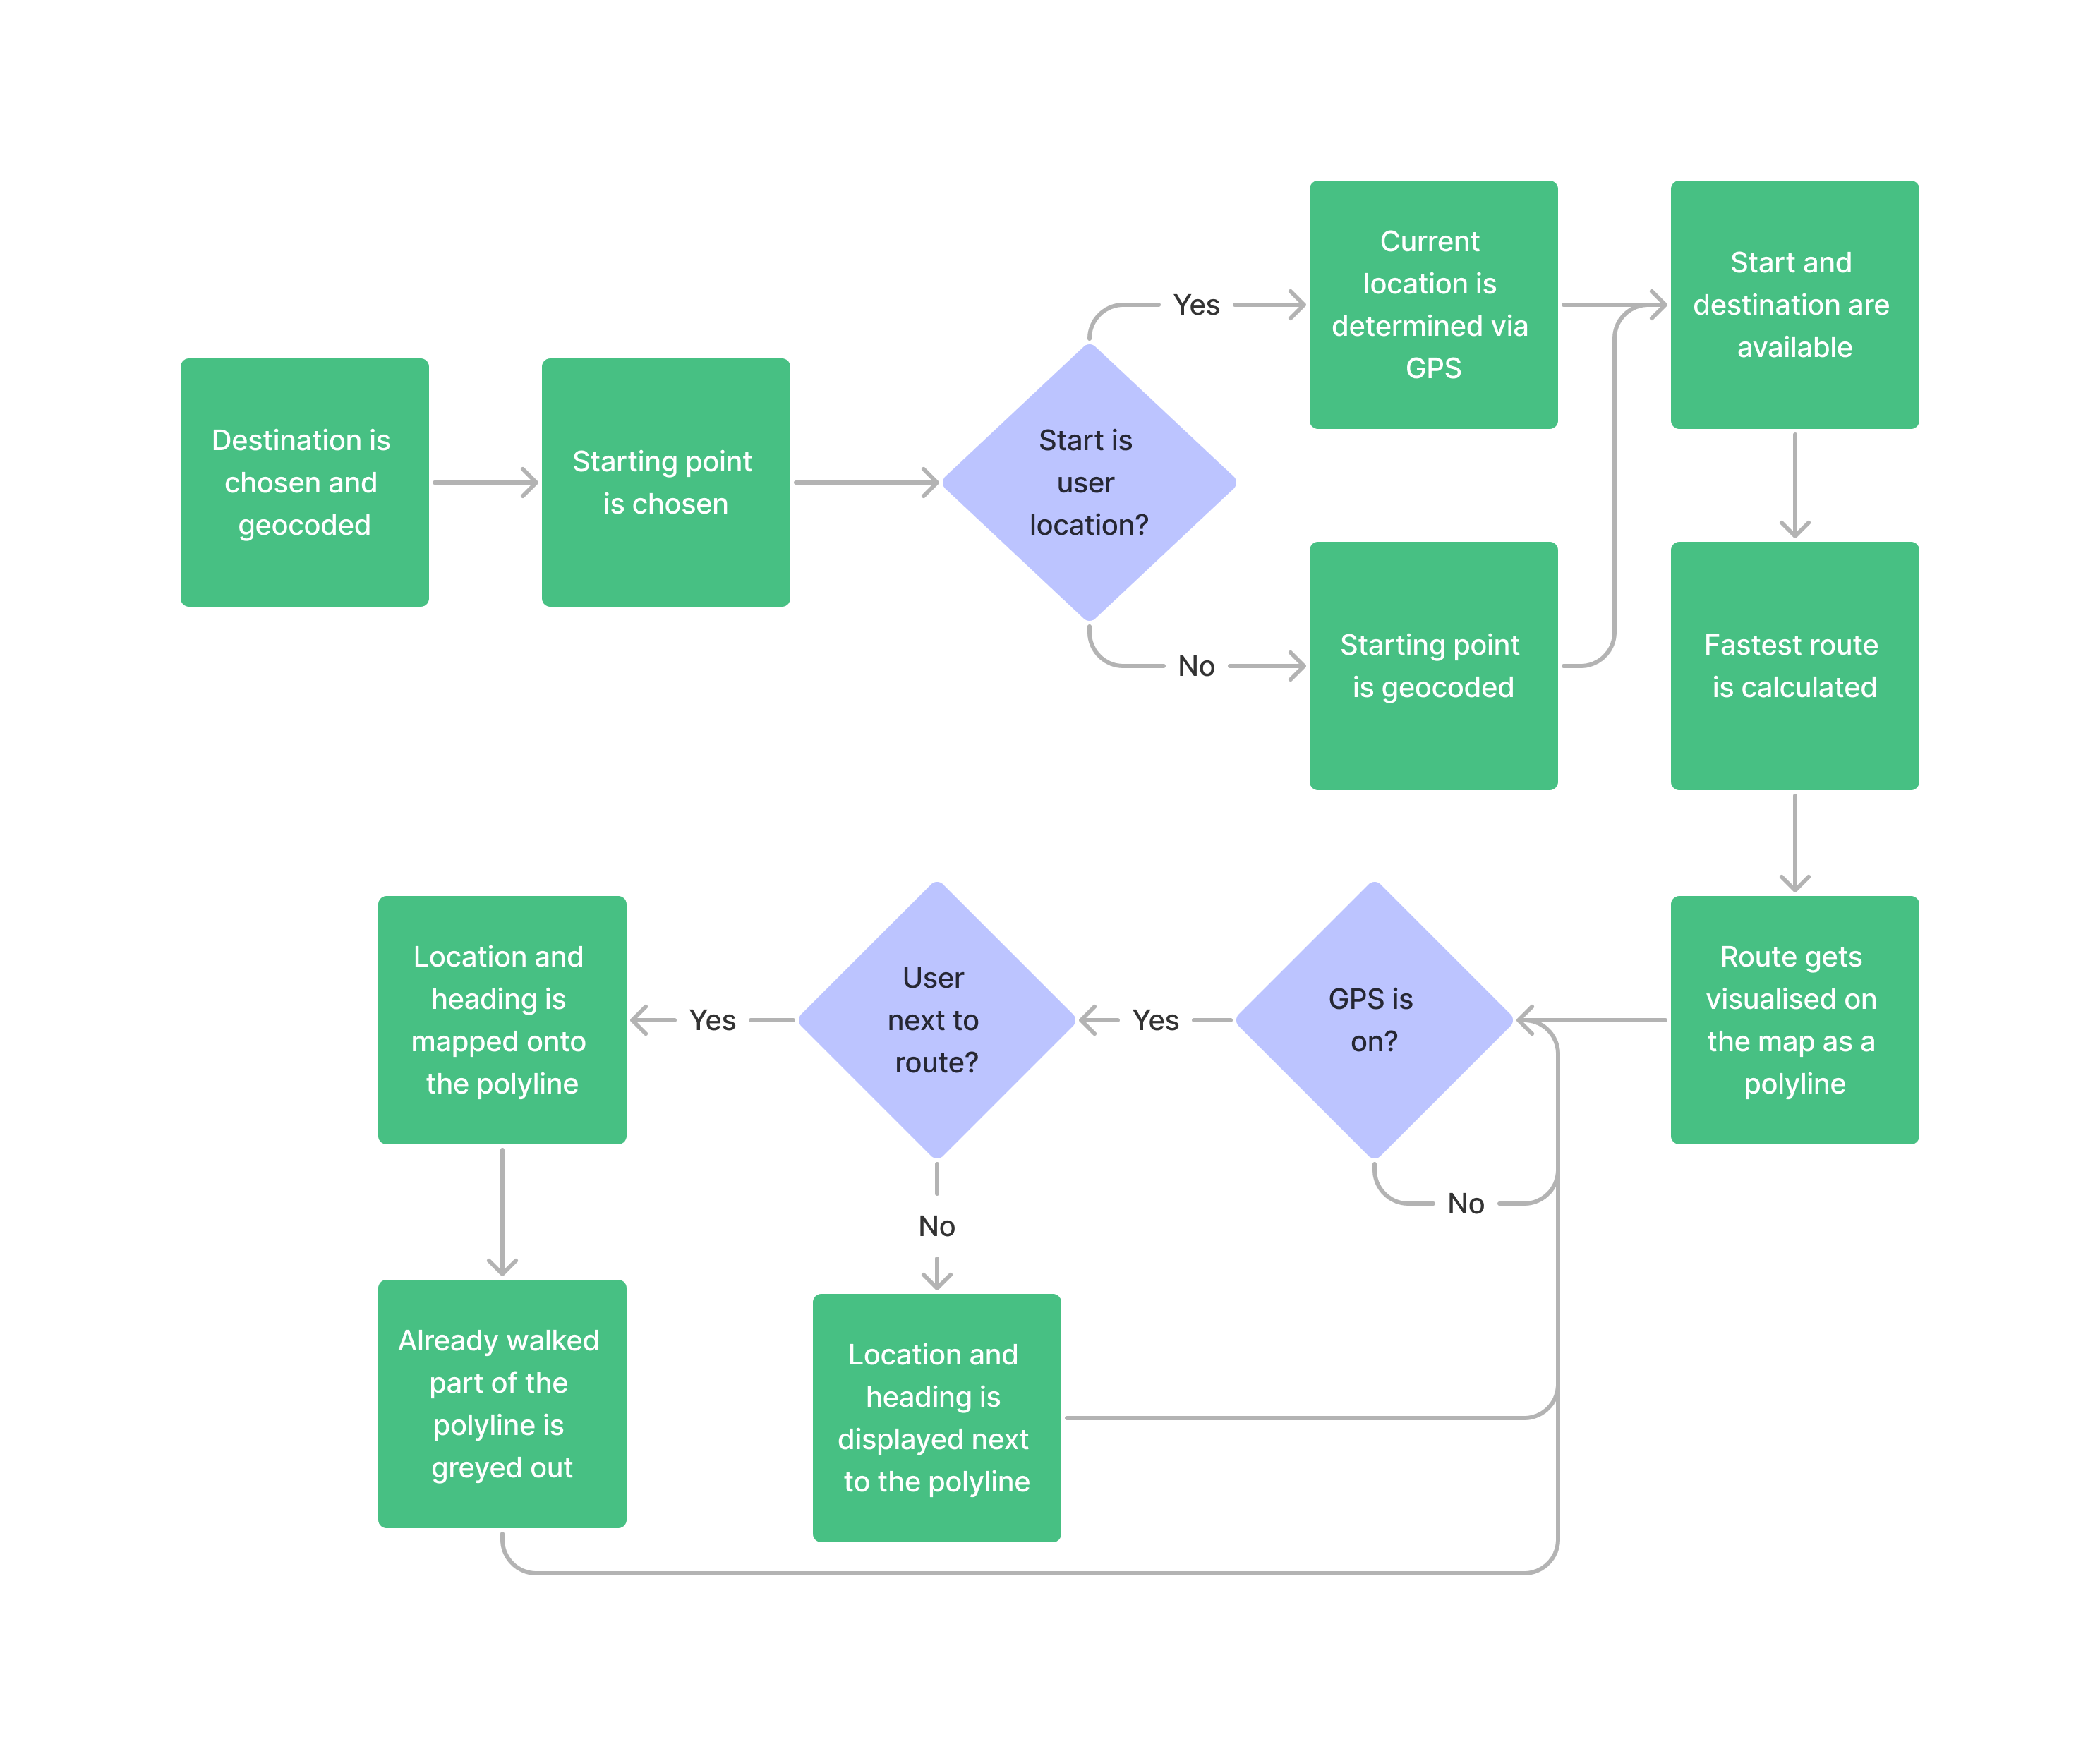
\includegraphics[width=0.85\textwidth]{images/navigation_process.png}\\
	\caption{Complete navigation system procedure}
\end{figure}

\subsection{Information layer}
An additional layer on top of the campus map consisting of location-based information is a natural addition to the feature set of the mobile app. It enhances the user experience, the relevance of the whole product and the overall digital information culture of TU Berlin by providing overlays, markers and labels filled with data about the campus.

This section provides a brief overview of the underlying data and technology used to provide the information on the layer.

There are three main sources, that are publicly available and relevant to the information layer. On the one hand, there is the official website of TU Berlin \cite{tu_berlin_main}, with sections for current events, the latest news, deadlines, etc. On the other hand, there is the MOSES system \cite{tu_berlin_moses} containing data about all the different courses, rooms and studies. A third relevant source of information is the website of Studierendenwerk Berlin \cite{studierendenwerk_berlin} with meal plans for its different canteens and a timetable for events.

Information is collected by downloading and parsing the content of respective websites. The data is further categorized and -if possible- mapped onto different POIs on the campus map (e.g., a canteen gets its meal plan assigned). This helps to provide an intuitive and organized presentation and access to the user.

The collected data can be categorized according to its timeliness and the intervals in which it has to be updated: General information about different fields of study, courses and rooms only changes by semester. This particular data can be retrieved once at the start of every semester and does not need daily live updates. It is also possible to supply it via app updates, instead of providing a direct in-app functionality for data retrieval. Data that gets updated regularly on the other hand, e.g., meal plans, events, news, etc. has to be always retrievable from the app.

The proposed solution for data collection and provision runs on a web server and consists of a web crawler for information retrieval, parsing and POI mapping, a CSV generator to convert the crawled information into a standardized and simple-to-use format and a REST API, that provides the client/mobile device the ability to retrieve the CSV files. The web crawler and CSV generator are both triggered periodically by several CRON jobs, whose timings are dependent on the timeliness of the crawled data. Due to its simplicity, the circumstance that there are no complex relations in the data and the fact that all room data from TU Berlin is provided in it, the CSV format is chosen as an alternative to a fully-fledged database system for data storage.

By splitting the logic for crawling and provision, the workload that arises on TU Berlin's and Studierendenwerk's websites from retrieving data can be limited to a minimum: The server only crawls data when an update is needed (e.g., weekly for meal plans), instead of loading and parsing the web resources on client request. Further advantages are the fact that loading times for requests from clients are independent of TU Berlin's and Studierendenwerk's infrastructure, that the language for web crawling can be chosen independently from the programming framework (in this case Python with its Selenium \cite{selenium} and BeautifulSoup \cite{beautifulsoup4} libraries are used) and that the web crawling logic can be changed without updating the app.

\begin{figure}[H]
	\centering
	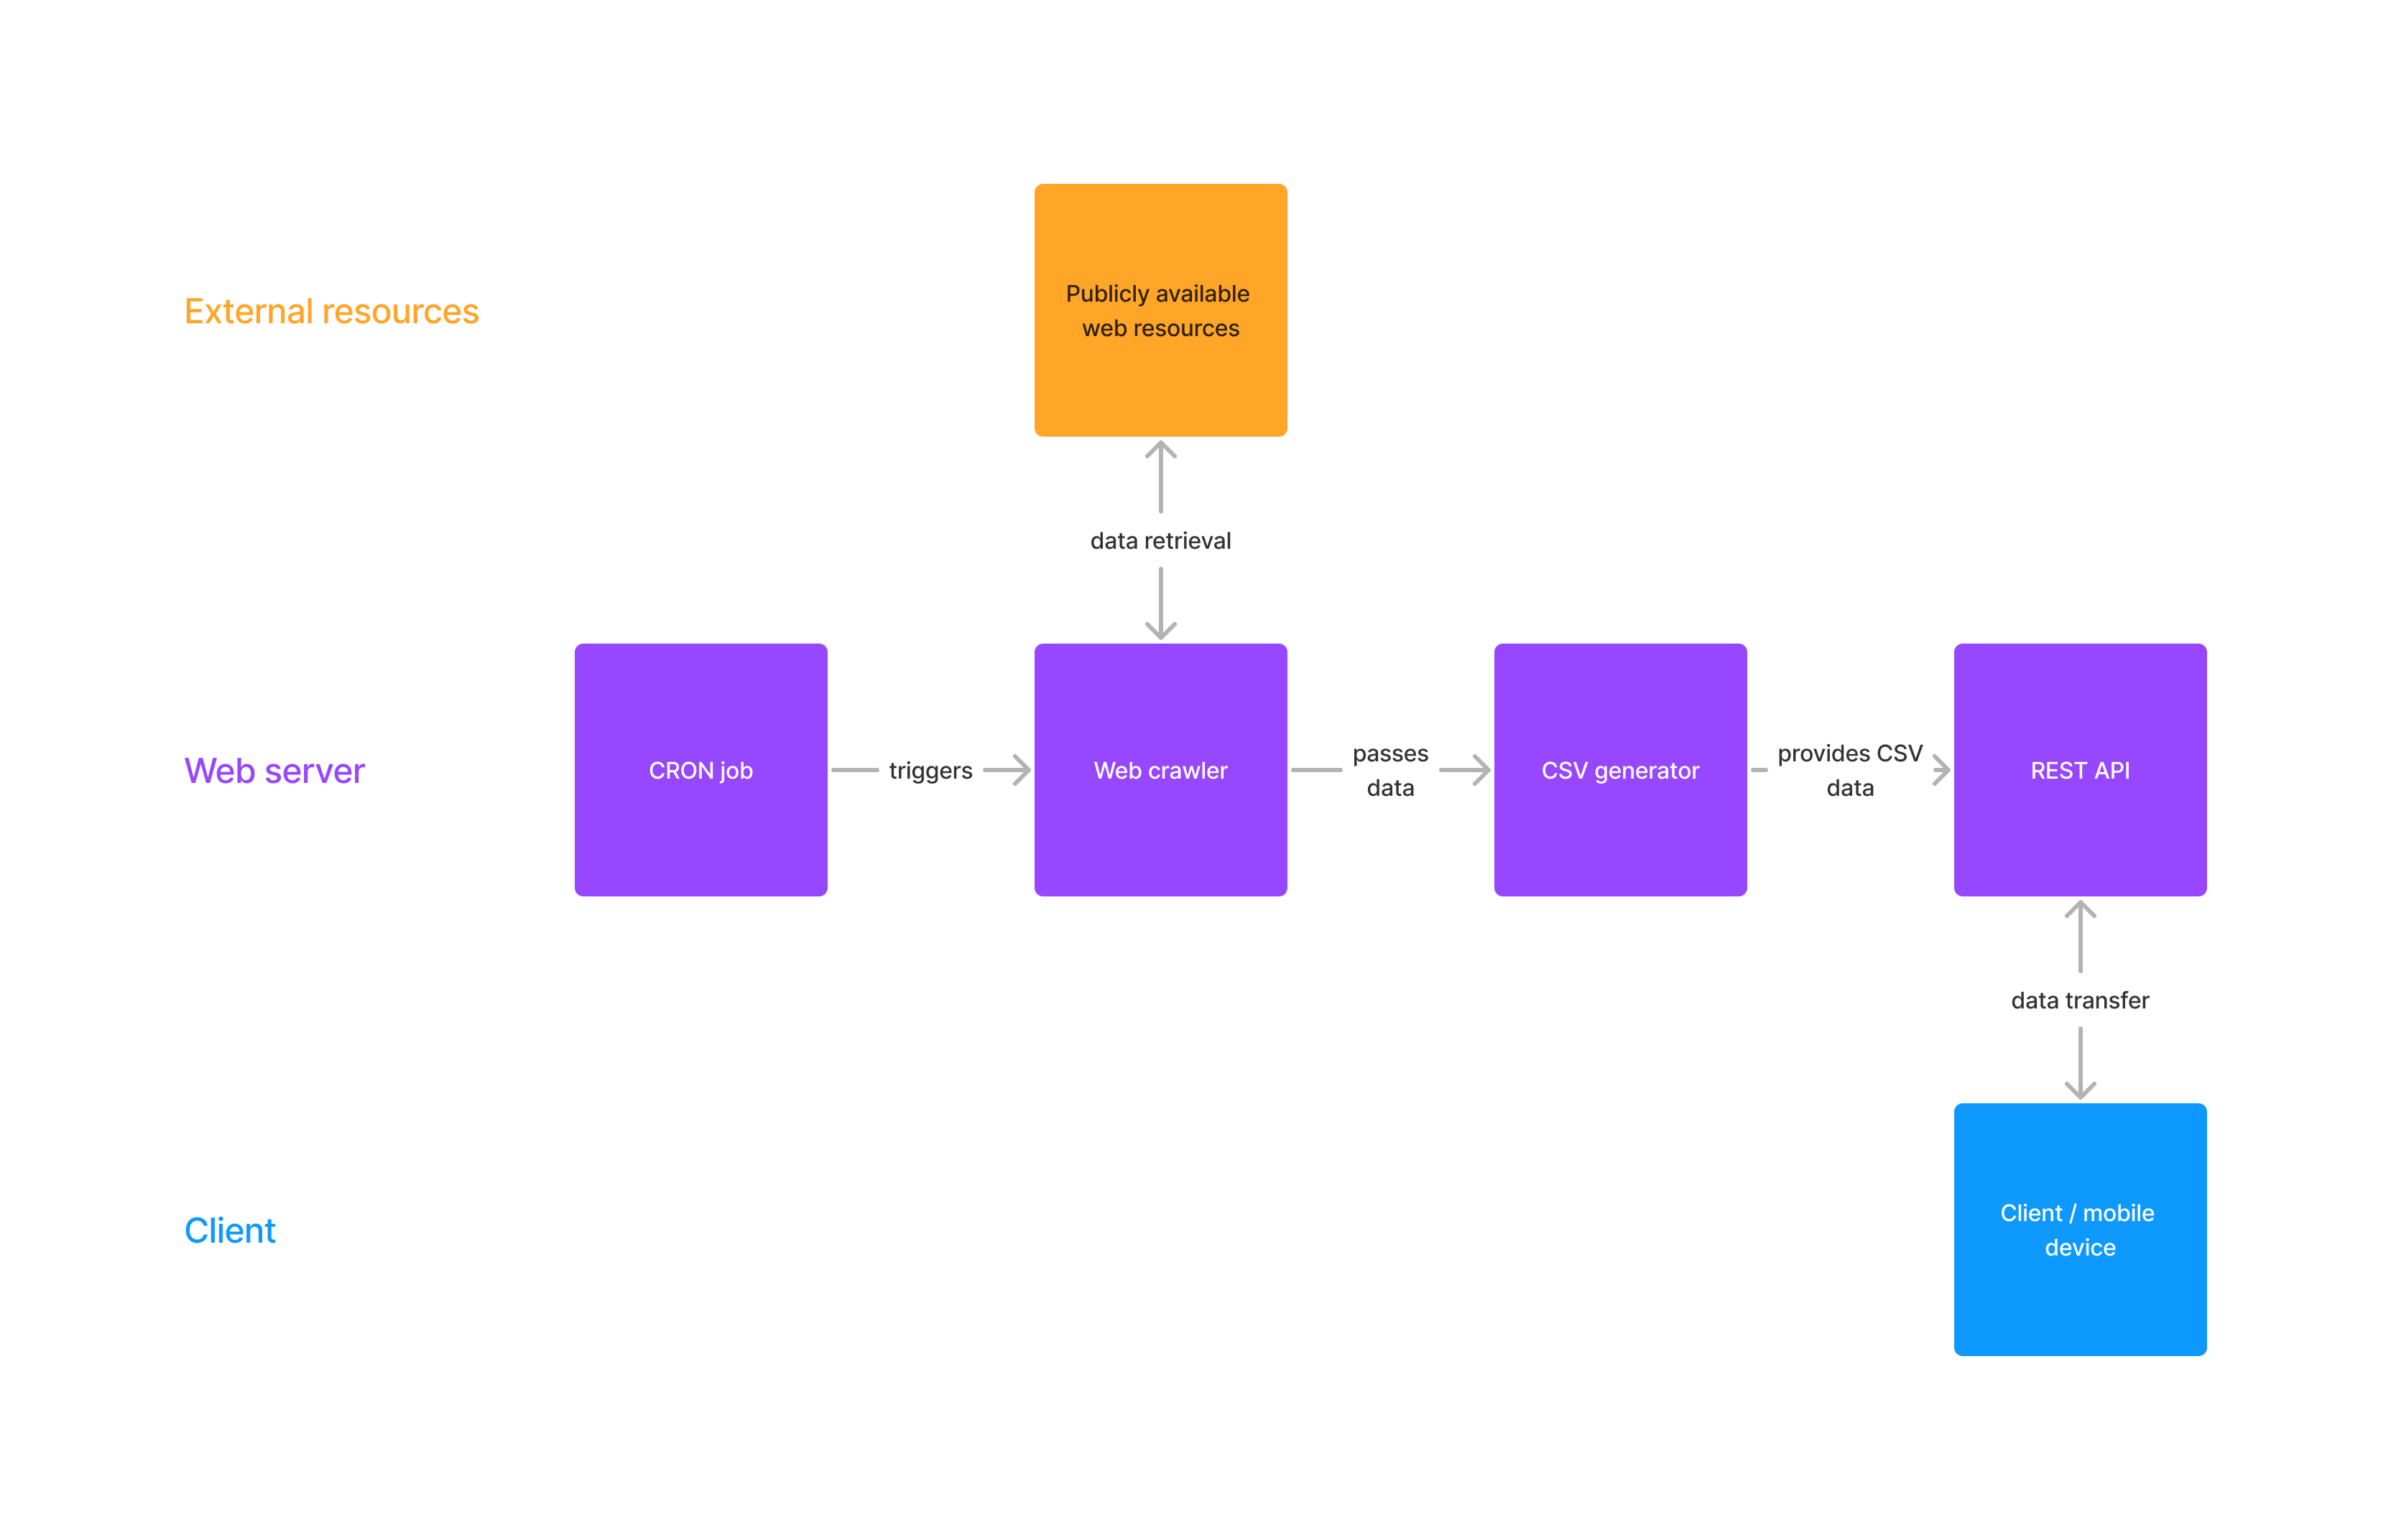
\includegraphics[width=0.85\textwidth]{images/information_layer_backend.png}\\
	\caption{Data retrieval process for the information layer}
\end{figure}

%\subsection{Exploration vs. search}
%\subsection{Search functionality}
%\subsection{Alternative presentation of information}

\subsection{Offline-first design}
One important aspect of the app concept is an extensive focus on offline usability. The whole system is designed to allow the user (as far as possible) a network-connection-free app usage. This applies in particular to the navigation system, the campus map and the information layer of the app:

Campus map: The campus map is locally implemented on the device. All necessary information can be therefore loaded and used without a network connection.

Navigation system: Due to the comparatively small scope of the navigation system, the weighted graph for navigation as well as the system for routing can both be implemented and executed on-device. Only the navigation feature working with live user location updates relies on stable GPS functionality.

Information layer: Loading and presenting information on TU Berlin's main campus requires access to the respected online resources and cannot be realized without a network connection. The need for network connectivity can be nevertheless reduced: Since no data requires real-time updates (the most critical data being meal plans that require weekly updates), the data for the information layer can be stored locally after download and loaded from memory for the remaining week. This approach reduces the need for internet connectivity to a minimum.

%This can be realized by sending silent push notifications at the start of every week. Devices that cannot receive the synchronizing push notification can download the data while being used. At best, this system allows the user to use the app throughout the week without going online.

\section{App development framework}
The choice of app development framework is an important step while conceptualizing and designing the product. It determines the programming language of the project, the built-in device- and system-specific capabilities that can be accessed during development as well as the performance of the app. It has to be selected in consideration of the project's requirements. The following enumeration presents the most important demands for this thesis:
\begin{itemize}
    \item Used technologies: Working with low-level hardware and operating system APIs is an important part of development. Technologies and systems used in the key features of the product (e.g., GPS capabilities) have to be accessible or implemented in the selected framework.
    \item Cross-platform capabilities: Native app development is complex and time-consuming. Learning and especially working with two different codebases (Java / Kotlin for Android, Swift / Obj. C for IOS) is difficult and not possible within the scope of this thesis. Cross-platform frameworks solve this problem by providing the ability to work with a single codebase for different operating systems.
    \item Execution speed: Regarding the fact that the whole navigation functionality has to take place locally on the phone, the speed with which the code of the mobile app gets executed is crucial to a responsive and fast user experience. Particularly the algorithms used for routing have to be reliably computable within seconds.
\end{itemize}

Based on the previously defined requirements, the Flutter framework \cite{flutter} is chosen for this work. In addition to its cross-platform capabilities, it also offers the ability to compile source code into platform-specific machine code for near-native execution performance. It further comes with access to thousands of packages through the dart package manager pub \cite{pub_dev}, an extensive set of pre-built components for user interfaces and the ability to write platform-specific code for low-level API access.

\section{User experience design}

\section{User interface design}